\chapter{Discussion}
Please tell more about conclusion and how to the next work of this study.

\section{Jesron Marudut Hatuan/1164077}
\subsection{Teori}
\begin{enumerate}
\item Mengapa file suara harus di lakukan MFCC.
\subitem Alasan mengapa File suara atau audio harus dilakukan MFCC  karena MFCC dapat mengubah file suara/frekuensi suara ke dalam sebuah bentuk data, yaitu menjadi data vektor yang nantinya dapat diolah menjadi sebuah output dimana telah dilakukan ekstraksi oleh MFCC selanjutnya direalisasikan sebagai data matrix. Contoh ilustrasi dapat dilihat pada gambar \ref{c6t_1}.
\begin{figure}[!htbp]
\centerline{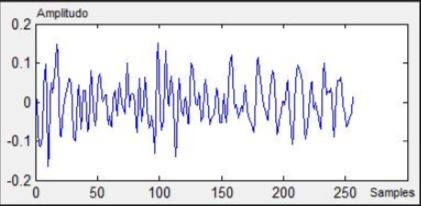
\includegraphics[width=1\textwidth]{figures/c6t/1.JPG}}
\caption{Suara ke MFCC}
\label{c6t_1}
\end{figure} 
\item Penjelasan tentang konsep dasar neural network.
\subitem Neural Network merupakan cara untuk menkomputasi yang efisien dimana tema utamanya dipinjam dari analogi jaringan saraf biologis. Neural Network juga biasa disebut dengan jaringan saraf tiruan dimana Neural Network sebenarnya dapat mengadopsi dari kemampuan otak manusia yang dapat memberikan rangsangan, melakukan proses, dan memberikan output. Contoh ilustrasi dapat dilihat pada gambar \ref{c6t_2}.
\begin{figure}[!htbp]
\centerline{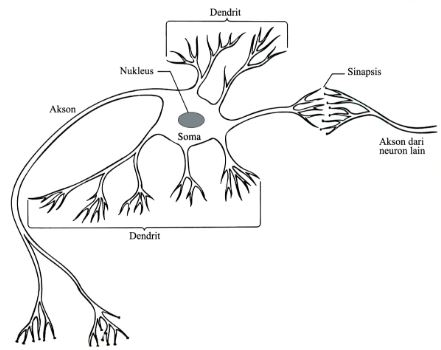
\includegraphics[width=1\textwidth]{figures/c6t/2.JPG}}
\caption{Neural Network}
\label{c6t_2}
\end{figure} 
\item Penjelasan tentang konsep dari pembobotan dalam neural network.
\subitem Neural Network dapat dikonfigurasi untuk aplikasi tertentu, seperti pengenalan pola atau klasifikasi data, contohnya saat Neural Network melakukan penyesuaian koneksi sinaptik antara Neuron, maka dilakukan dengan menyesuaikan nilai bobot yang ada pada setiap konektivitas baik dari input, Neuron maupun output disinkronkan dengan penyesuaian koneksi sinaptik antar neuron itu sendiri. Contoh ilustrasi dapat dilihat pada gambar \ref{c6t_3}.
\begin{figure}[!htbp]
\centerline{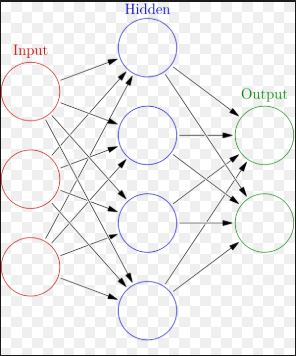
\includegraphics[width=1\textwidth]{figures/c6t/3.JPG}}
\caption{Konsep Pembobotan pada Neural Network}
\label{c6t_3}
\end{figure} 
\item Penjelasan tentang konsep fungsi aktifasi dalam Neural Network.
\subitem Dalam Neural Network, fungsi aktivas adalah setiap Neuron dapat mempunyai tingkat aktivasi yang merupakan fungsi dari input yang masuk padanya. Aktivasi yang dikirim suatu Neuron ke Neuron lain berupa sinyal dan hanya dapat mengirim sekali dalam satu waktu, meskipun sinyal tersebut disebarkan pada beberapa neuron yang lain. Contoh ilustrasi dapat dilihat pada gambar \ref{c6t_4}.
\begin{figure}[!htbp]
\centerline{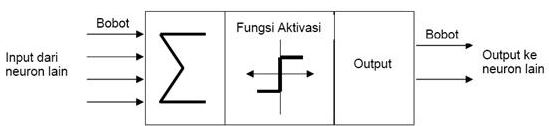
\includegraphics[width=1\textwidth]{figures/c6t/4.JPG}}
\caption{Fungsi Aktivasi pada Neural Network}
\label{c6t_4}
\end{figure} 
\item Penjelasan cara membaca hasil plot dari MFCC.
\subitem Cara membaca dari MFCC yaitu nanti akan ada outputan berbentuk grafik setelah melakukan plot dari MFCC. Kemudian terdapat frekuensi/Hz pada suara frekuensi biasanya vertikal atau biasa disimbolkan dengan sumbu y, Lalu terdapat waktu yang mana waktu diartikan dalam simbol sumbu x. Sedangkan pada bagian dalam dapat disimbolkan dengan sumbu z yang merupakan power atau kekuatan dari lagu atau suara atau audio yang dihasilkan. Untuk warna biru itu merupakan suara rendah, yang merah merupakan tinggi apabila daya frekuensi nya misalkan suara siul berarti dominan warna merah karena siul biasanya pada nada yang tinggi sedangkan jika bass dominan biru karena bass merupakan nada rendah. Contoh ilustrasi dapat dilihat pada gambar \ref{c6t_5}.
\begin{figure}[!htbp]
\centerline{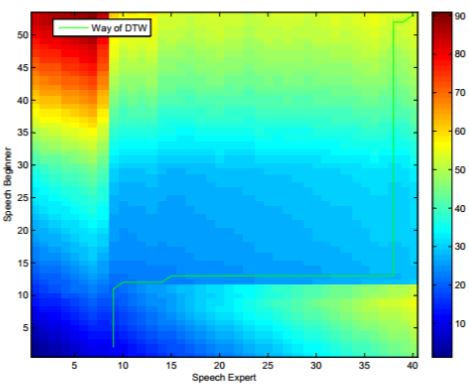
\includegraphics[width=1\textwidth]{figures/c6t/5.JPG}}
\caption{Membaca Hasil Plot dari MFCC}
\label{c6t_5}
\end{figure} 
\item Penjelasan tentang apa itu one-hot encoding.
\par One-hot encoding yaitu sebuah caraa untuk representasi data dari variabel kategori sebagai vektor biner. Yaitu nilai kategorika harus dipetakan ke nilai integer. Selanjutnya, setiap nilai integer direpresentasikan sebagai vektor biner yang semuanya bernilai nol kecuali indeks integer, yang dapat ditandai dengan 1. Contoh ilustrasi dapat dilihat pada gambar \ref{c6t_6}.
\begin{figure}[!htbp]
\centerline{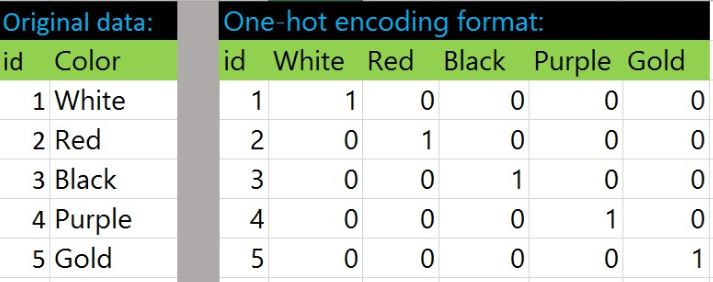
\includegraphics[width=1\textwidth]{figures/c6t/6.JPG}}
\caption{One-Hot Encoding}
\label{c6t_6}
\end{figure} 
\item Penjelasan fungsi dari np.unique dan to\_categorical dalam kode program.
\begin{itemize}
\item np.unique adalah cara untuk mengekstaksi elemen-elemen unik tertentu yang terdapat dalam array.
\item sedangkan to\_categorical adalah cara untuk mengubah vektor kelas yang berupa integer menjadi matriks kelas biner.
\end{itemize}
\begin{figure}[!htbp]
\centerline{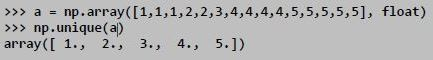
\includegraphics[width=1\textwidth]{figures/c6t/7.JPG}}
\caption{np.unique}
\end{figure} 
\begin{figure}[!htbp]
\centerline{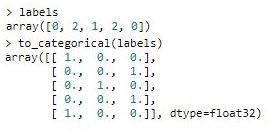
\includegraphics[width=1\textwidth]{figures/c6t/7_1.JPG}}
\caption{to\_categorical}
\end{figure} 
\item Penjelasan fungsi dari Sequential dalam kode program.
\subitem Fungsi dari Sequential dalam kode program yaitu sebuah jenis model yang dapat digunakan dalam perhitungan ataupun code program yang dapat direalisasikan. Neural Networks Sequential dapat membangun fitur tingkat tinggi melalui lapisan yang berurutan. Sequential juga merupakan proses dimana membandingkan setiap elemen larik satu per satu secara beruntun, mulai dari elemen pertama, sampai dengan elemen terakhir atau elemen yang dicari sudah ditemukan.  Contoh ilustrasi dapat dilihat pada gambar \ref{c6t_8}.
\begin{figure}[!htbp]
\centerline{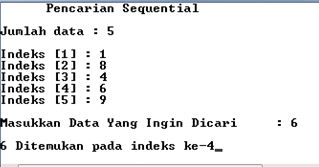
\includegraphics[width=1\textwidth]{figures/c6t/8.JPG}}
\caption{One-Hot Encoding}
\label{c6t_8}
\end{figure} 
\end{enumerate}